\chapter{Seismic data fundamentals}\label{ch:data}

\section{From ground motion to numbers}
A seismometer converts ground motion into an electrical signal. The Raspberry Shake 3D carries three orthogonal
geophones, nominally with a natural frequency of $f_0 = 4.5$~Hz, one vertical (Z) and two horizontal (N--S and E--W).
A geophone is a coil suspended in the field of a magnet fixed to the case. When the ground, and with it the case,
moves, the coil lags behind by inertia, and the relative velocity between coil and magnet induces a voltage
proportional to that \emph{relative velocity}. Above its natural frequency the relative velocity of the coil equals
the ground velocity, so the voltage is proportional to ground velocity in the pass band
(Chapter~\ref{ch:response} derives the transfer function; \textcite{havskov2016} treat the physics in depth).

The analogue voltage is then amplified and digitised by an analogue-to-digital converter (ADC). The integers it
produces are called \emph{counts}. A count is not a physical unit: one count corresponds to a fixed number of
volts, and, through the sensor, to a frequency-dependent velocity. The conversion is the subject of
Chapter~\ref{ch:response}.

\section{Sampling and the Nyquist frequency}
The ADC measures the signal at regular intervals $\dt$, giving samples $x[n]=x(n\,\dt)$. The Raspberry Shake 3D
samples at $\fs = 100$~samples per second, so $\dt = 10$~ms. The sampling theorem states that a band-limited signal
can be reconstructed exactly from its samples if and only if it contains no energy at or above the
\emph{Nyquist frequency}
\begin{equation}
  \fN = \frac{\fs}{2} = 50\ \text{Hz}.
\end{equation}
Energy above $\fN$ does not vanish when sampled: it \emph{aliases}, folding back into the band below $\fN$. A
sinusoid of frequency $f$ with $\fN < f < \fs$ produces exactly the same samples as one of frequency $\fs - f$
(\cref{fig:alias}). Aliasing cannot be undone after sampling, so digitisers apply an analogue and digital
\emph{anti-alias filter} before and during decimation; its roll-off is visible as a fall in the spectra of RS3D
near $\fN$ (Chapter~\ref{ch:noise}). Consequently the top few hertz of any RS3D spectrum are attenuated by the
instrument, not by the ground.

\begin{figure}[tbp]
\centering
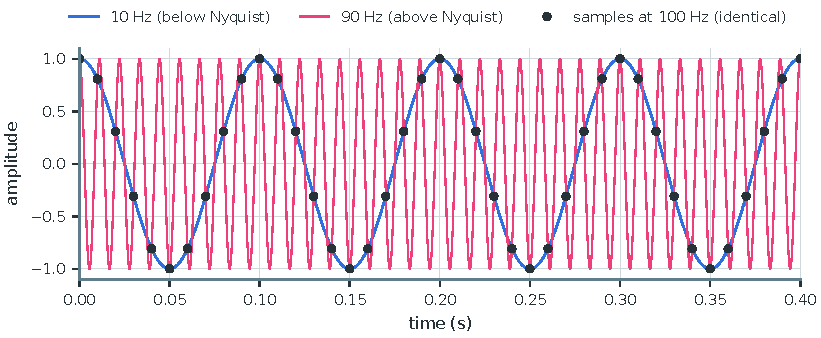
\includegraphics[width=\linewidth]{theory-aliasing}
\caption{Aliasing. At $\fs = 100$~Hz a 90~Hz cosine (pink) and a 10~Hz cosine (blue) have identical samples
(dots). Because $90 = \fs - 10$, the faster signal is indistinguishable from the slower one after sampling.}\label{fig:alias}
\end{figure}

\begin{rs3dkey}
Everything the application shows lies below $\fN = 50$~Hz, and the last few hertz below it are shaped by the
Shake's anti-alias filter.
\end{rs3dkey}

\section{Channel naming}
Every stream of samples is identified by four codes, the SEED identifier \parencite{fdsnseed2012}:
\begin{center}\ttfamily\small
\begin{tabular}{@{}llll@{}}
\textcolor{rs3dgrey}{network} & \textcolor{rs3dgrey}{station} & \textcolor{rs3dgrey}{location} & \textcolor{rs3dgrey}{channel}\\
AM & R77A7 & 00 & EHZ
\end{tabular}
\end{center}
\code{AM} is the Raspberry Shake network, \code{R77A7} the station, \code{00} the location code. The three-letter
channel code is itself structured: \code{E} is the \emph{band} code (an extremely short-period instrument sampled at
80~Hz or more), \code{H} the \emph{instrument} code (a high-gain seismometer), and the last letter the
\emph{orientation}: \code{Z} vertical, \code{N} north--south, \code{E} east--west. An RS3D therefore serves
\code{EHZ}, \code{EHN} and \code{EHE}. The application sorts channels vertical-first (\code{Z}, \code{N}, \code{E})
so that the default channel is always the vertical.

\section{miniSEED and the day archive}
Seismic samples are exchanged as \emph{miniSEED}, a sequence of fixed-length records (512 bytes is typical for
SeedLink). Each record carries the four identifier codes, the time of its first sample, the sampling rate, and a block
of samples stored as first differences compressed with the Steim algorithm. Because consecutive samples of a smooth
signal differ by small amounts, the compression is lossless and efficient. One channel-day is 8.64~million samples,
about 35~MB as raw 32-bit integers; the Shake's compressed archive for all three channels takes about 85~MB per
day (the figure quoted in the application's own storage help).

A \emph{gap} is a place where a record's start time does not continue the previous record. Readers such as ObsPy
split a stream at gaps into separate \emph{traces}; the application keeps them separate (and shows them as breaks
or blank columns) rather than inventing data. How gaps are measured is the subject of Chapter~\ref{ch:quality}.

Files are arranged in the \emph{SeisComP data structure} (SDS), one file per channel per day:
\begin{center}
\code{<root>/YEAR/NET/STA/CHAN.D/NET.STA.LOC.CHAN.D.YEAR.DOY}
\end{center}
where \code{DOY} is the day of the year, zero-padded to three digits. For example the vertical channel of
15~October 2026 is stored in \file{2026/AM/R77A7/EHZ.D/AM.R77A7.00.EHZ.D.2026.288}. The Shake keeps the same layout
under \file{/opt/data/archive}, and the application mirrors it on the laptop, so a file downloaded from the Shake
can be used unchanged.

\begin{rs3dapp}
\file{core/store.py} implements the day-file layout (\code{day\_path}, \code{days}, \code{load}); \code{import\_file}
splits any miniSEED file into day files, merging with data already present so that importing the same file twice
changes nothing. \file{core/archive.py} copies day files from the Shake: it downloads into a temporary \file{.part}
file and renames it only when complete, so an interrupted transfer never looks like a finished day, and it
always re-fetches the newest remote day because the Shake is still writing to it.
\end{rs3dapp}

\section{Time}
Sample times are UTC. The time of sample $n$ of a record starting at $t_0$ is $t_0 + n/\fs$. The accuracy of
$t_0$ depends entirely on the Shake's clock, which is kept right by the network time protocol; an offset of
100~ms is already visible when two stations are compared. The Status page therefore flags a clock offset above
100~ms as a warning and above 1000~ms as an error (\file{core/status.py}). Leap seconds are not modelled:
timestamps are POSIX-style seconds, which is adequate for the minute-to-second resolution the application targets.
